Handwritten text databases come in numerous flavours and purposes. Among the simplest ones are isolated character datasets, the largest one being the NIST database, consisting of over 800,000 binary images of carefully segmented characters \cite{Juan}. The MNIST database that derives from it only contains handwritten digits and is a popular ground for measuring model performances, as well as an intuitive didactic tool \cite{Juan}. Other datasets feature particular aspects like different resolutions and normalization techniques (TICH) or including other characters like punctuation (COUT) \cite{Juan}.

Nevertheless, the most interesting datasets are definitely those whose smallest working unit is the word, not the character \cite{Juan}. A well known instance is the IAM dataset, which represents the work of around 400 writers producing together 1066 written forms with over 82,000 words \cite{IAM}. The dataset offers builtin word, line and paragraph segmentation (figure \ref{FigIAMExterpt}), in addition to other parameters related to the writing style, such as the slant or the stroke width \cite{IAM}.

\begin{figure}[htbp]
    \centering
        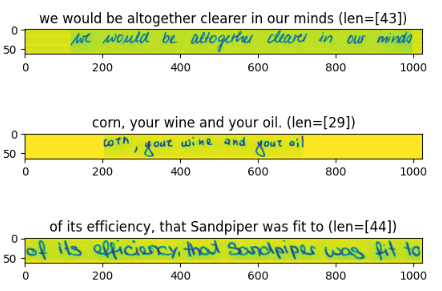
\includegraphics[scale=0.7]{figures/IAM_preview}
    \caption{An exterpt from the IAM lines dataset}
    \label{FigIAMExterpt}        
\end{figure}

A great workload of the current thesis is based on the IAM dataset due to its accesibility and ease of use. It is notable to know that IAM is a way to clean comparing to how people usually write texts. Real life applications often do not encounter almost horizontal text lines separated by generous spaces \cite{Juan}. However, proper data preprocessing may cope with these issues, and IAM dataset still remains a powerful image-text source for training HTR models. There are also other valuable non-English datasets like RIMES (French) \cite{Juan}, Osborne (Spanish) \cite{Juan}, KHATT (Arabic) \cite{msdoctrlite}. Moreover, we remind historical sources datasets like Esposalles \cite{msdoctrlite} or the ICDAR2017 dataset \cite{icdar}. Tables \ref{sota_IAM} and \ref{sota_RIMES} show state-of-the-art results on the IAM and RIMES datasets.

It is worth mentioning that some researchers are providings ways to enhance small sized datasets by using a generative model to build new data based on the existing samples. While the usage of GANs \cite{ganText} or Variational Auto-Encoders \cite{vaeText} may be well suited to the task, the literature comes up with an interesting method based on capsule networks (CapsNet), a notorious example being TextCaps \cite{textcaps}.

\begin{table}[htbp]
\begin{center}
\begin{tabular}
{|p{170pt}|p{100pt}|}
\hline
 Model  &  CER\cite{cer} \\
\hline 
TrOCR-large 558M \cite{trocr} & 2.89\% \\ \hline
Transformer+CNN \cite{trcnn} & 2.96\% \\ \hline
TrOCR-base 334M \cite{trocr} & 3.42\% \\ \hline
TrOCR-small 62M \cite{trocr} & 4.22\% \\ \hline
Easter2.0 \cite{easter20} & 6.21\% \\ \hline
\end{tabular}
\end{center}
\captionsetup{justification=centering,margin=1cm}
\caption{State of the art on IAM dataset (fullpage)}
\label{sota_IAM}
\end{table}

\begin{table}[htbp]
\begin{center}
\begin{tabular}
{|p{220pt}|p{90pt}|}
\hline
 Model  &  CER\cite{cer} \\
\hline 
Start,Follow,Read (fullpage)\cite{sfr} & 2.1\% \\ \hline
MDLSTM+CTC (fullpage)\cite{mdlstm_rimes} & 2.5\% \\ \hline
CNN+BiGRU (word)\cite{mdlstm_rimes} & 2.65\% \\ \hline

\end{tabular}
\end{center}
\captionsetup{justification=centering,margin=1cm}
\caption{State of the art on RIMES dataset}
\label{sota_RIMES}
\end{table}


